%%%%%%%%%%%%%%%%%%%%%%%%%%%%%%%%%%%%%%%%%
% Structured General Purpose Assignment
% LaTeX Template
%
% This template has been downloaded from:
% http://www.latextemplates.com
%
% Original author:
% Ted Pavlic (http://www.tedpavlic.com)
%
% Note:
% The \lipsum[#] commands throughout this template generate dummy text
% to fill the template out. These commands should all be removed when 
% writing assignment content.
%
%%%%%%%%%%%%%%%%%%%%%%%%%%%%%%%%%%%%%%%%%

%----------------------------------------------------------------------------------------
%   PACKAGES AND OTHER DOCUMENT CONFIGURATIONS
%----------------------------------------------------------------------------------------

\documentclass{article}

\usepackage{fancyhdr} % Required for custom headers
\usepackage{lastpage} % Required to determine the last page for the footer
\usepackage{extramarks} % Required for headers and footers
\usepackage{graphicx} % Required to insert images
\usepackage{lipsum} % Used for inserting dummy 'Lorem ipsum' text into the template

\usepackage[T1]{fontenc} % Codificación de las fuentes utilizadas
\usepackage[spanish]{babel} % Español como idioma principal del texto (permite hyphenation de palabras al final de una línea)
\selectlanguage{spanish}
\usepackage{hyperref}
\hypersetup{
	colorlinks=true,
	urlcolor=blue,
	linkcolor=blue,
	citecolor=blue
}
\usepackage{listings}
\usepackage{float}

% Margins
\topmargin=-0.45in
\evensidemargin=0in
\oddsidemargin=0in
\textwidth=6.5in
\textheight=9.0in
\headsep=0.25in 

\linespread{1.1} % Line spacing

% Set up the header and footer
\pagestyle{fancy}
%\lhead{\hmwkAuthorName} % Top left header
%\chead{\hmwkTitle\ (\hmwkClassInstructor): \hmwkTitle} % Top center header
%\rhead{\firstxmark} % Top right header
%\lfoot{\lastxmark} % Bottom left footer
%\cfoot{} % Bottom center footer
%\rfoot{Page\ \thepage\ of\ \pageref{LastPage}} % Bottom right footer
\renewcommand\headrulewidth{0.4pt} % Size of the header rule
\renewcommand\footrulewidth{0.4pt} % Size of the footer rule

\setlength\parindent{0pt} % Removes all indentation from paragraphs

%----------------------------------------------------------------------------------------
%   DOCUMENT STRUCTURE COMMANDS
%   Skip this unless you know what you're doing
%----------------------------------------------------------------------------------------

% Header and footer for when a page split occurs within a problem environment
\newcommand{\enterProblemHeader}[1]{
\nobreak\extramarks{#1}{#1 continued on next page\ldots}\nobreak
\nobreak\extramarks{#1 (continued)}{#1 continued on next page\ldots}\nobreak
}

% Header and footer for when a page split occurs between problem environments
\newcommand{\exitProblemHeader}[1]{
\nobreak\extramarks{#1 (continued)}{#1 continued on next page\ldots}\nobreak
\nobreak\extramarks{#1}{}\nobreak
}

\setcounter{secnumdepth}{0} % Removes default section numbers
\newcounter{homeworkProblemCounter} % Creates a counter to keep track of the number of problems

\newcommand{\homeworkProblemName}{}
%\newenvironment{homeworkProblem}[1][Problem \arabic{homeworkProblemCounter}]{ % Makes a new environment called homeworkProblem which takes 1 argument (custom name) but the default is "Problem #"
\newenvironment{homeworkProblem}[1][Evaluación \arabic{homeworkProblemCounter}]{
\stepcounter{homeworkProblemCounter} % Increase counter for number of problems
\renewcommand{\homeworkProblemName}{\large{#1}} % Assign \homeworkProblemName the name of the problem
\section{\large{\homeworkProblemName}} % Make a section in the document with the custom problem count
\enterProblemHeader{\homeworkProblemName} % Header and footer within the environment
}{
\exitProblemHeader{\homeworkProblemName} % Header and footer after the environment
}

\newcommand{\problemAnswer}[1]{ % Defines the problem answer command with the content as the only argument
\noindent\framebox[\columnwidth][c]{\begin{minipage}{0.98\columnwidth}#1\end{minipage}} % Makes the box around the problem answer and puts the content inside
}

\newcommand{\homeworkSectionName}{}
\newenvironment{homeworkSection}[1]{ % New environment for sections within homework problems, takes 1 argument - the name of the section
\renewcommand{\homeworkSectionName}{#1} % Assign \homeworkSectionName to the name of the section from the environment argument
\subsection{\homeworkSectionName} % Make a subsection with the custom name of the subsection
\enterProblemHeader{\homeworkProblemName\ [\homeworkSectionName]} % Header and footer within the environment
}{
\enterProblemHeader{\homeworkProblemName} % Header and footer after the environment
}
   
%----------------------------------------------------------------------------------------
%   NAME AND CLASS SECTION
%----------------------------------------------------------------------------------------

\newcommand{\hmwkTitle}{Configuración de un sistema de compilación multiplataforma con distcc y aplicación de este en un entorno distribuido} % Assignment title
\newcommand{\hmwkDueDate}{Martes,\ 21\ de\ April\ de\ 2015} % Due date
\newcommand{\hmwkAuthorName}{Diego Martín Arroyo} % Your name

%----------------------------------------------------------------------------------------
%   TITLE PAGE
%----------------------------------------------------------------------------------------

% \title{
% \vspace{2in}
% \textmd{\textbf{\hmwkTitle}}\\
% \normalsize\vspace{0.1in}\small{Realizado\ el\ \hmwkDueDate}\\
% \vspace{0.1in}\large{\textit{\hmwkClassInstructor\ }}
% \vspace{3in}
% }

\title{\hmwkTitle}
\author{\textbf{\hmwkAuthorName}}
\date{21 de abril de 2015}

%----------------------------------------------------------------------------------------

\begin{document}

\maketitle

%----------------------------------------------------------------------------------------
%   TABLE OF CONTENTS
%----------------------------------------------------------------------------------------

\setcounter{tocdepth}{1}

\newpage
\tableofcontents
\newpage


\section{Introducción}

Uno de los graves inconvenientes a la hora de desarrollar software para el sistema distribuido es la pequeña capacidad de cómputo individual de cada nodo. Si bien esta circunstancia no supone un inconveniente significativo a la hora la ejecución, supone un grave obstáculo a la hora de realizar procesos de compilación, en particular, de paquetes de software voluminosos, tales como pueden ser bibliotecas de código, cuyo tiempo de compilación en una Raspberry Pi puede alcanzar varias horas.

Diversas soluciones han sido propuestas para solucionar este problema, siendo una de las más simples y efectivas la compilación cruzada. Un compilador cruzado es capaz de generar código ejecutable en el juego de instrucciones de otra máquina, permitiendo aprovechar las ventajas de otro equipo (en particular la mayor capacidad de cálculo) para agilizar el proceso de compilación. En el caso concreto del sistema, el equipo compilador cuenta con un procesador de arquitectura i686 con una capacidad de cómputo muy superior al del chip ARM presente en los nodos del sistema. Conseguir realizar compilaciones en este equipo facilitaría el trabajo de administración del sistema, la instalación de nuevo \textit{software} e incluso el desarrollo de código.

\section{crostool-ng}

Crosstool-ng\footnote{Existe una amplia cantidad de información sobre el proyecto en su sitio web, \href{http://crosstool-ng.org/}{crosstool-ng.org}} es una utilidad para la generación de cadenas de herramientas (\textit{toolchains}) tales como GCC \textit{GNU Compiler Collection}, que permiten compilar y enlazar códigos fuente. El proyecto tiene como objetivo crear \textit{toolchains} ajustadas a cada necesidad específica, ofreciendo un gran número de parámetros de configuración con el objetivo de optimizar al máximo el proceso de compilación y adaptarse a las necesidades de los usuarios. \textbf{Crosstool-ng} es un proyecto cuyo origen se remonta a la herramienta crosstool de Daniel Kegel\footnote{\href{http://kegel.com/crosstool/}{http://kegel.com/crosstool/}}.

\subsection{Configuración de crosstool-ng}

La configuración de crosstool-ng es sencilla una vez se conocen los diferentes parámetros a tener en cuenta. Para poder realizar compilaciones en nuestro sistema es necesario un \textit{toolchain} con las siguientes características:

\begin{itemize}
	\item Capaz de compilar en la arquitectura \textbf{ARMv7} de 32 bits con alineamiento de bits \textit{little endian}. El procesador de la Raspberry implementa operaciones con números en coma flotante en el \textit{hardware}, por lo que es posible aprovechar esta característica en los programas a compilar.
	\item Un compilador de C
	\item Compilador de C++
	\item Compilador de FORTRAN (Opcional)
	\item Bibliotecas estándar (librería estándar)
\end{itemize}

Para crear este compilador es necesario realizar los siguientes pasos:

\begin{enumerate}
	\item Descarga de los archivos desde el sitio del proyecto \footnote{\href{www.crosstool-ng.org/download/crosstool-ng}{www.crosstool-ng.org/download/crosstool-ng}}. El compilador se ha creado con la versión \textbf{1.20.0}, la más reciente durante la creación de este documento, publicada el 8 de septiembre de 2014.
	\item Instalación de las dependencias de \textbf{crosstool-ng}:\\
		\texttt{gawk bison flex gperf cvs texinfo automake libtool ncurses-dev g++ subversion python-dev libexpat1-dev cmake}
	\item Descomprimir el fichero y realizar la configuración del mismo con \texttt{./configure --prefix=/opt/cross} (el directorio de compilación puede ser modificado). Ejecutar el comando \texttt{make} y \texttt{make install}.
	\item Añadir a la variable \texttt{PATH} la ruta \texttt{/opt/cross/bin}.
	Una vez realizados estos pasos la herramienta queda instalada y se podrá crear \textit{toolchains}.
	\item Crear un directorio en el que se almacenarán los diferentes archivos auxiliares durante el proceso de creación del compilador.
	\item Ejecutar \texttt{ct-ng menuconfig}, que presentará una serie de opciones en un panel interactivo:

	\begin{itemize}
		\item En la opción \textit{Paths and misc options}, activar la opción ``Enable Try features marked as EXPERIMENTAL'', y modificar el valor \textit{Number of parallel jobs} a un valor menor o igual al doble de núcleos presentes en el procesador del servidor. También es posible modificar el directorio de despliegue.
		\item En el menú \textit{Target options}, seleccionar ``arm'' como \textit{Target architecture} \textit{bitness} como 32 bit y \textit{Endianness} como \textit{Little endian}
		\item \textit{Operating System}: Linux
		\item Elegir la opción estable de \textit{Binutils version} más reciente en el menú \textit{Binutils}
		\item Elegir la opción para \textit{gcc} \textit{linaro} cuya versión sea más reciente en el menú \textit{C Compiler}. Activar además la compilación para los lenguajes \textbf{C++}, \textbf{FORTRAN} y \textbf{Java} si se desea.
		\item Activar la opción \textit{gdb} en \textit{Debug Facilities}.
	\end{itemize}
	\item Una vez realizados estos pasos es necesario ejecutar el comando \texttt{ct-ng build} que generará el conjunto de herramientas. El proceso de creación ha llegado a requerir una hora de procesado. Tras el proceso de compilación se contará con los ejecutables en el directorio \texttt{/opt/cross/x-tools/arm-unknown-linux-gnueabi/bin} o en aquella ruta especificada.

\end{enumerate}
%la máquina

\subsection{Alternativas}

En los archivos adjuntos a la documentación se encuentra un \textit{toolchain} generado para sistemas Linux en arquitecturas i386 y x86\_64, así como los archivos de configuración para la creación de los mismos.

%En caso de utilizar
En el caso de utilizar Arch ARM y la arquitectura del equipo a utilizar como compilador sea x86\_64 es posible descargar los parámetros de configuración desde la web del proyecto Arch Linux ARM o los propios ejecutables precompilados\footnote{Archivos .config:
\begin{itemize}
\item ARMv5: \href{http://archlinuxarm.org/mirror/development/ct-ng/xtools-dotconfig-v5}{archlinuxarm.org/mirror/development/ct-ng/xtools-dotconfig-v5}
\item ARMv6: \href{http://archlinuxarm.org/mirror/development/ct-ng/xtools-dotconfig-v6}{archlinuxarm.org/mirror/development/ct-ng/xtools-dotconfig-v6}
\item ARMv7: \href{http://archlinuxarm.org/mirror/development/ct-ng/xtools-dotconfig-v7}{archlinuxarm.org/mirror/development/ct-ng/xtools-dotconfig-v7}
\end{itemize}
\textit{Toolchains precompilados}:
\begin{itemize}
\item ARMv5 \textit{soft float}: \href{http://archlinuxarm.org/builder/xtools/x-tools.tar.xz}{http://archlinuxarm.org/builder/xtools/x-tools.tar.xz}
\item ARMv6 \textit{hard float}: \href{http://archlinuxarm.org/builder/xtools/x-tools6h.tar.xz}{http://archlinuxarm.org/builder/xtools/x-tools6h.tar.xz}
\item ARMv7 \textit{hard float}: \href{http://archlinuxarm.org/builder/xtools/x-tools7h.tar.xz}{http://archlinuxarm.org/builder/xtools/x-tools7h.tar.xz}
\end{itemize}
También es posible utilizar el paquete \textbf{distccd-alarm}, que realiza todos los pasos necesarios para instalar \textbf{distccd} para todas las arquitecturas de forma simplificada. Únicamente válido para sistemas \textbf{Arch Linux} ejecutados en una arquitectura x86\_64: \href{https://github.com/WarheadsSE/PKGs/tree/master/distccd-alarm}{github.com/WarheadsSE/PKGs/tree/master/distccd-alarm}.
}.

\subsection{Uso}

Ejemplo de ejecución:

\begin{lstlisting}[language=bash]
$ arm-unknown-linux-gnueabi-gcc --version
arm-unknown-linux-gnueabihf-gcc (crosstool-NG 1.20.0) 4.9.2
arm-unknown-linux-gnueabihf-gcc main.c -o main
$
\end{lstlisting}

\subsection{Integración con un entorno de desarrollo}

Es posible integrar el compilador cruzado en un entorno de desarrollo integrado como \textbf{Eclipse}\footnote{\href{http://eclipse.org/}{http://eclipse.org/}}, siguiendo la siguiente secuencia de pasos. Es necesario contar con los \textit{plugins} \textbf{C/C++ Development Tools}, \textbf{C/C++ Development Tools SDK} y \textbf{C/C++ GCC Cross Compiler Support}.

\begin{enumerate}
\item Creación de un nuevo proyecto para el lenguaje elegido (es importante que se haya creado el compilador para ese lenguaje), indicando que el tipo de compilador será cruzado (opción \textbf{Cross GCC}). Se deben seleccionar las opciones de configuración para el desarrollo en la siguiente ventana..

\begin{figure}[H]
\centering
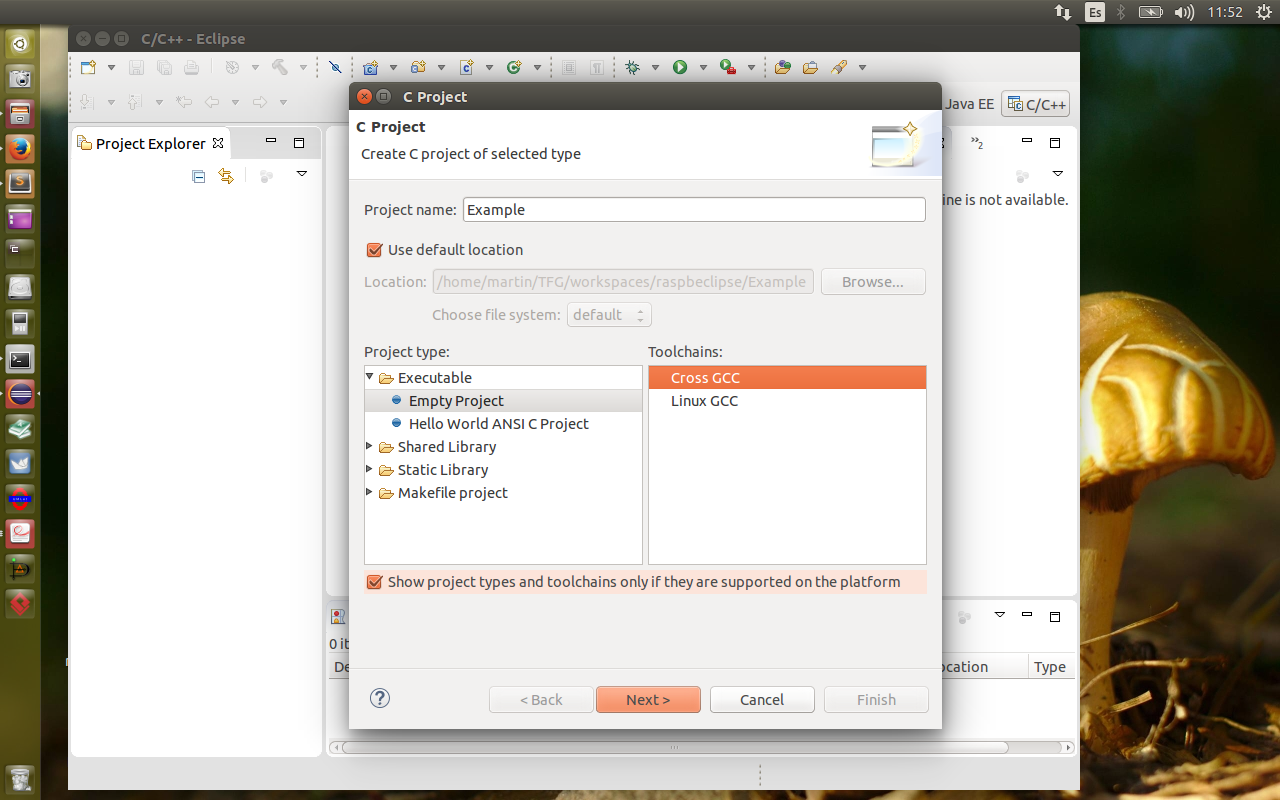
\includegraphics[width=0.7\textwidth]{Recursos/raspbeclipse/projectcreation}
\end{figure}
\begin{figure}[H]
\centering
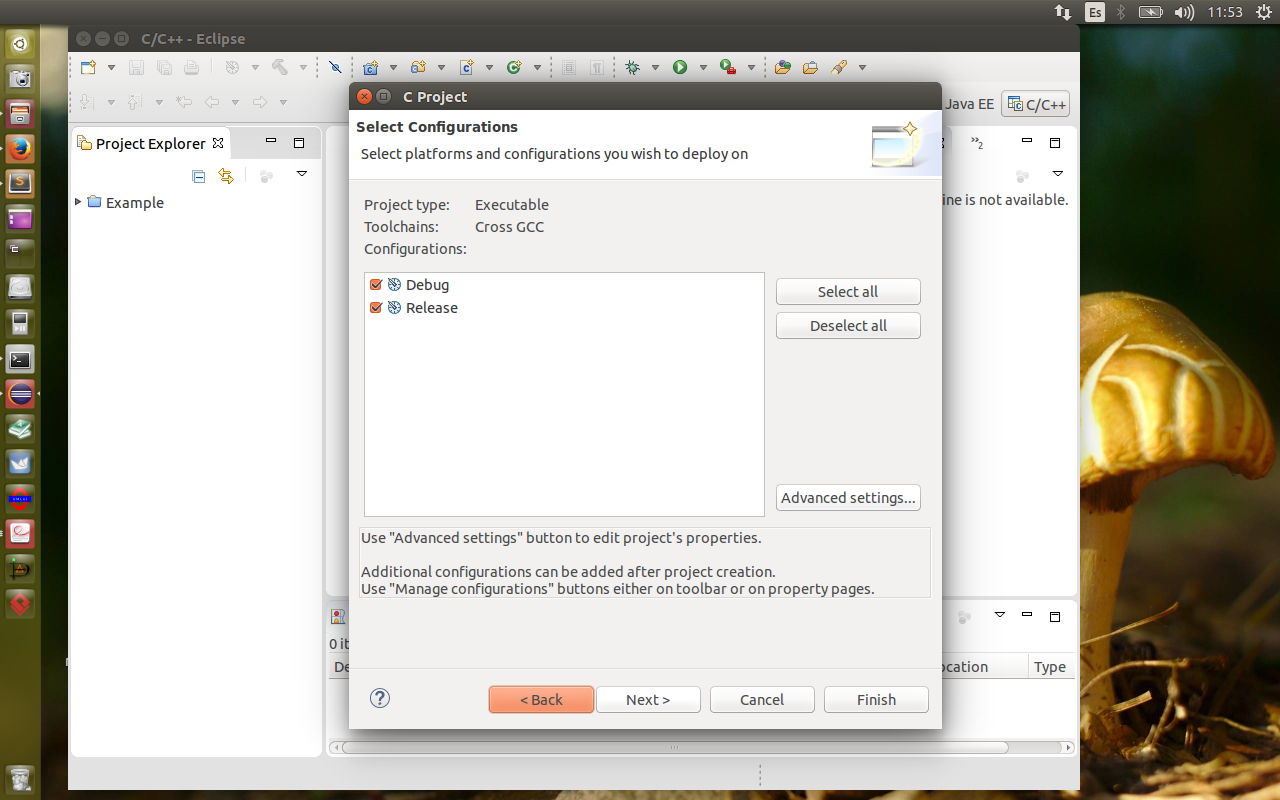
\includegraphics[width=0.7\textwidth]{Recursos/raspbeclipse/configurations}
\end{figure}

\item Definición de la ruta del compilador.

Se especifican la ruta donde se encuentran los diferentes ejecutables del compilador, indicando el prefijo que les acompaña (Eclipse realizará una llamada convencional al compilador como si se tratase de un proyecto típico, por lo que para identificar cada uno de los ejecutables, se debe indicar dicho prefijo, si lo hay). En este caso, dado que se han creado enlaces simbolicos que no incluyen el prefijo, no es necesario indicarlo.
\begin{figure}[H]
\centering
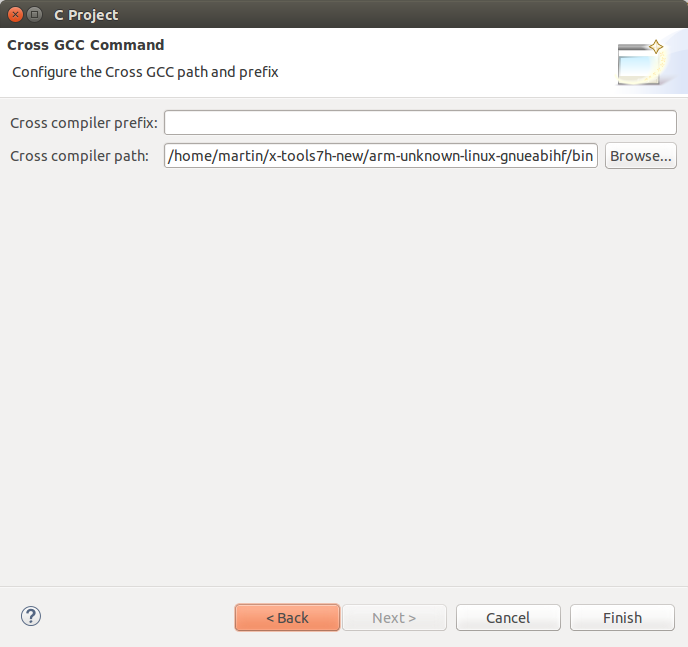
\includegraphics[width=0.5\textwidth]{Recursos/raspbeclipse/compilerpath}
\end{figure}

\item Creación del código y compilación.

Se añaden o crean los archivos a compilar y se ejecuta la acción \textbf{Build}. La consola mostrará el resultado de la operación.

\begin{figure}[H]
\centering
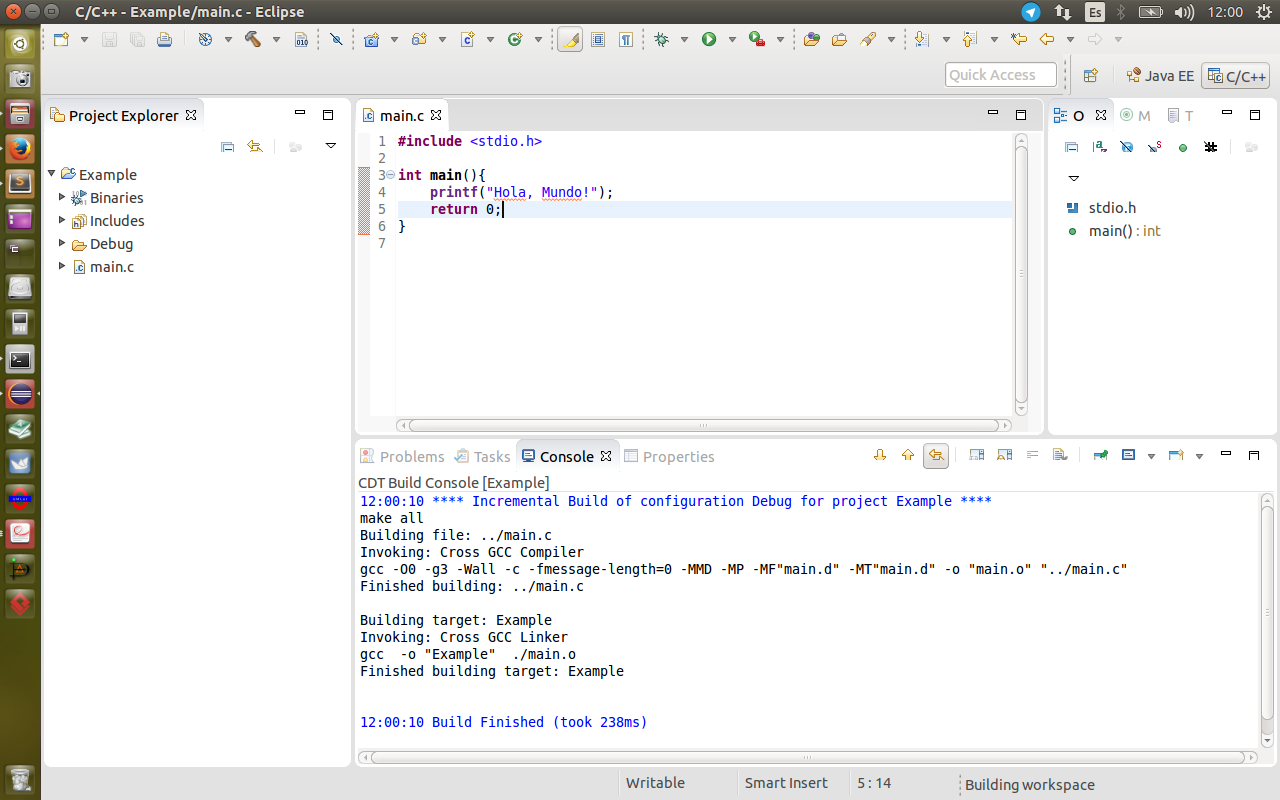
\includegraphics[width=0.7\textwidth]{Recursos/raspbeclipse/build}
\end{figure}

\item Evaluación del resultado.

Utilizando la herramienta \textbf{file} es posible verificar la arquitectura del ejecutable.

\begin{figure}[H]
\centering
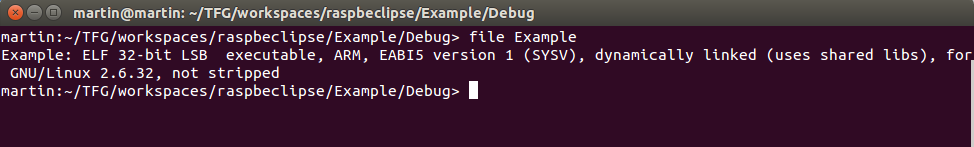
\includegraphics[width=0.7\textwidth]{Recursos/raspbeclipse/result}
\end{figure}

\end{enumerate}
%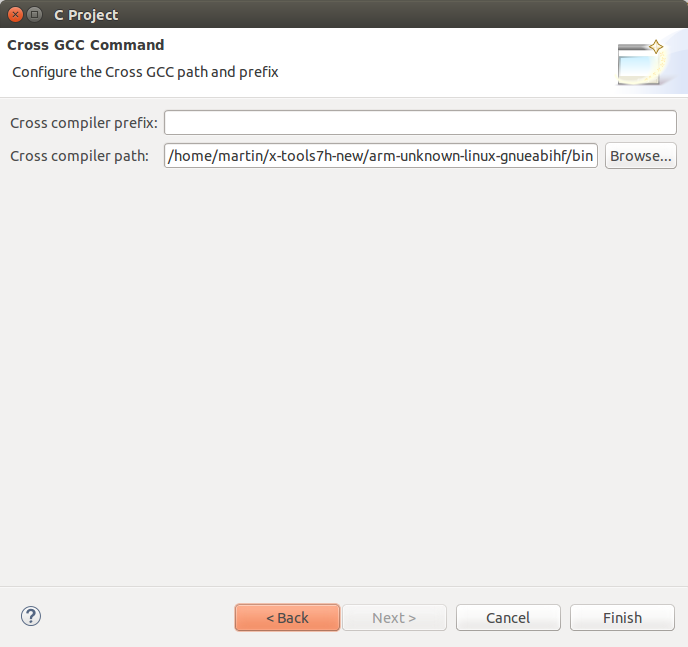
\includegraphics{Recursos/raspbeclipse/compilerpath}

%http://elinux.org/Raspberry_Pi_Kernel_Compilation
%http://getglitched.com/?page_id=253


%Fuente: http://archlinuxarm.org/developers/distcc-cross-compiling


%https://lists.samba.org/archive/distcc/2009q2/003918.html
%https://www.raspberrypi.org/forums/viewtopic.php?f=51&t=60908
%http://www.robopgmr.com/?p=2959
%http://stackoverflow.com/questions/19162072/installing-raspberry-pi-cross-compiler
\section{distcc}

La compilación distribuida consiste en una serie de máquinas dedicadas a realizar procesos de compilación comandadas por una serie de nodos denominados maestros, que envían una serie de instrucciones de compilado a la máquina remota para que sean ejecutadas, retornando el resultado de dicho proceso de compilación. Distcc es una herramienta que actúa como demonio del sistema, escuchando peticiones de compilación de forma continua.

\section{Problemas conocidos}

Muchas de las versiones de \textbf{crosstool-ng} presentes en su repositorio presentan problemas debido a que los archivos que necesita descargar ya no se encuentran disponibles. La versión utilizada en el sistema es la 1.20.0, liberada el 8 de septiembre de 2014.

En ocasiones el repositorio subversion de EGlibC presenta un error en la descarga, debido a la sobrecarga de su servidor. En este caso es necesario utilizar Glibc como biblioteca estándar para C. Además, el desarrollo de Eglibc ha sido interrumpido, debido a que los desarrolladores del proyecto consideran que los objetivos del mismo ya han sido cumplidos y se han integrado en Glibc, por lo que es recomendable utilizar esta versión en futuras versiones del compilador.

%http://www.eglibc.org/faq
%http://www.eglibc.org/mission
%http://www.eglibc.org/home 28/04
%http://crosstool-ng.org/download/crosstool-ng/

%http://hertaville.com/2012/09/28/development-environment-raspberry-pi-cross-compiler/
%http://hertaville.com/2014/04/12/cross-compiling-qt4-app/
%TODO: tiempos de compilación

%http://archlinuxarm.org/developers/distributed-compiling
%http://johnlane.ie/a-distcc-server-for-raspberry-pi.html
% https://wiki.debian.org/Distcc
% http://wiki.vpslink.com/HOWTO:_Install/Configure_Distcc
% http://www.kegel.com/crosstool/
% https://code.google.com/p/distcc/
% http://elinux.org/Toolchains
% http://es.wikipedia.org/wiki/Cadena_de_herramientas
% http://es.wikipedia.org/wiki/Linux_From_Scratch
% http://es.wikipedia.org/wiki/GNU_toolchain
% http://getglitched.com/?page_id=253

\nocite{bootccrosstool}
\nocite{pointcloudscrosstool}
\nocite{linuxjournaldistcc}
\nocite{distccreference}
\nocite{distccfaq}
\nocite{jeremynicolacrosstool}
\nocite{mborgersoncrosstool}

\label{Bibliography}
\lhead{\emph{Bibliografía}}  % Change the left side page header to "Bibliography"
\bibliographystyle{ieeetr}  % Use the "unsrtnat" BibTeX style for formatting the Bibliography
\bibliography{distcc}  % The references (distcc) information are stored in the file named "distcc.bib"

\end{document}
